\documentclass[12pt, letterpaper, titlepage]{article}

% Packages
% Set margins
\usepackage[margin=1 in]{geometry}
% No page numbers
\usepackage{nopageno}
% Compact lists
\usepackage{paralist}
% Code blocks¬
\usepackage{listings}
% Custom colors
\usepackage{xcolor}
% Include images
\usepackage{graphicx}
% Table placement
\usepackage{float}
% Citations
\usepackage{cite}
% Math packages
\usepackage{amsmath, amssymb, amsfonts}
\usepackage{algorithmic}
% Allow verb in captions
\usepackage{cprotect}
% Fancy header
\usepackage{fancyhdr}
% Sub-figures
\usepackage{subfigure}
% Check for known extensions instead of the first dot
\usepackage{grffile}
% CSV tables
\usepackage{csvsimple}

% Color definitions
\definecolor{codegreen}{rgb}{0,0.6,0}
\definecolor{codegray}{rgb}{0.5,0.5,0.5}
\definecolor{codepurple}{rgb}{0.58,0,0.82}
\definecolor{backcolour}{rgb}{1.0,1.0,1.0}

% Code listing style¬
\lstdefinestyle{mystyle}{
  backgroundcolor=\color{backcolour},
  commentstyle=\color{codegreen},
  keywordstyle=\color{magenta},
  numberstyle=\tiny\color{codegray},
  stringstyle=\color{codepurple},
  basicstyle=\ttfamily\footnotesize,
  breakatwhitespace=false,
  breaklines=true,
  captionpos=b,
  keepspaces=false,
  numbersep=5pt,
  showspaces=false,
  showstringspaces=false,
  showtabs=false,
  tabsize=2
}
\lstset{style=mystyle}

% Definitions for spellings and consistency
% References
\newcommand{\figRef}[1]{Figure \ref{#1}}
\newcommand{\tabRef}[1]{Table \ref{#1}}
\newcommand{\eqRef}[1]{(\ref{#1})}

% Spellings
\newcommand{\ubu}{Ubuntu}
\newcommand{\ubuVer}{18.04 64-bit}
\newcommand{\kali}{Kali Linux}
\newcommand{\vb}{VirtualBox}
\newcommand{\metasploit}{Metasploit}
\newcommand{\msfv}{MSFvenom}
\newcommand{\payloadName}{TCP bind shell}
\newcommand{\mibex}{MiBeX}
\newcommand{\mibexFull}{\mibex{}: Malware-inserted Benign Datasets for Explainable Machine Learning}

% Quantities
\newcommand{\benignFiles}{1103}
\newcommand{\totalFiles}{2206}
\newcommand{\usableFiles}{1794}
\newcommand{\maxFileSize}{100 KB}
\newcommand{\imageWidth}{32}
\newcommand{\imageHeight}{3070}
\newcommand{\maxTrainingEpochs}{5000}
\newcommand{\batchSize}{32}
\newcommand{\learningRate}{0.001}
\newcommand{\trainPercent}{80\%}
\newcommand{\testPercent}{20\%}
\newcommand{\trainAccuracy}{100.0\%}
\newcommand{\testAccuracy}{99.72\%}

% Custom math operators
\DeclareMathOperator*{\argmax}{arg\,max}

% Set header
\setlength\headheight{14pt}
\pagestyle{fancy}
\fancyhf{}
\chead{\small \mibexFull{}}
\cfoot{\small \thepage}

\begin{document}
\begin{titlepage}
  \centering
  \par \normalsize \textsc{
    A capstone project submitted to the Department of Electrical Engineering
    and Computing Systems (DEECS) at the University of Cincinnati
  }
  \vfill
  \par \rule{\linewidth}{2pt}
  \LARGE
  \par \mibex{}: Malware-inserted Benign Datasets
  \par for Explainable Machine Learning
  \par \rule{\linewidth}{2pt}
  \vfill
  \Large
  \par \textit{Wayne Stegner}
  \vfill
  \normalsize
  \par \today
  \vfill
  \par 
\includegraphics[width=6cm]{Images/UC_Logo.eps}
  \vfill
  \normalsize
  \par Submitted in partial fulfillment of the degree of
  \par Bachelor of Science in
  \par Computer Engineering
  \vfill
  \begin{tabular}{p{3cm}p{6cm}p{1cm}p{3cm}}
    Wayne Stegner: & \hrulefill & Date: & \hrulefill\\
    \\
    Dr. Rashmi Jha: & \hrulefill & Date: & \hrulefill\\
  \end{tabular}
\end{titlepage}

\section*{Acknowledgments}
\par I would like to thank the following individuals for their contributions to this project.
Without you, this project would not have been possible.

\begin{itemize}
  \item The Design Knowledge Company, Dayton, Ohio and Air Force Research Laboratory, Wright Patterson, Ohio for funding this project under Award \# AFRL FA8650-18-C-1191.
  \item Dr. Rashmi Jha for your advisory expertise and guidance on the direction and scope of the project.
  \item AFRL associates Dr. David Kapp, Dr. Tem Kebede, and Daniel Koraneck for constructive technical discussion and your guidance on the scope of the project.
  \item Tyler Westland for sharing your knowledge of Linux, Makefile, and helping me troubleshoot my \msfv{} issues.
  \item Bayley King for giving me advice on training my Malware as Image classifier.
\end{itemize}

\pagebreak

\tableofcontents
\listoffigures
\listoftables

\pagebreak

\section{Abstract}
\par In the task of malware detection the method of machine learning has shown high accuracy in distinguishing malicious software from benign software.¬
As malware classification using machine learning shows more promise, it is desirable to extract explanations from the algorithms to validate the reasoning behind the decisions.¬
Santacroce et al. \cite{SantacroceMaV, SantacroceSalience} has studied the use of class saliency maps to extract features deemed malicious by malware classification neural networks.¬
However, current malware datasets do not have specific labeled malicious features, so validating the correctness of the extracted malicious features was impractical.¬

% Problem statement/Specific purpose¬
\par This work explored a method to produce a scalable malware dataset with intelligible malicious features for the purpose of evaluating explanations from machine learning malware classifiers.¬

% Methodology¬
First, I collected a pool of benign executable files from the \verb|/bin/| and \verb|/usr/bin/| directories of a default installation of \ubu{} \ubuVer{}, forming the benign group of the dataset.¬
Next, I used \msfv{} from the \metasploit{} framework in conjunction with the \verb|make| utility to insert a \payloadName{} Trojan payload into each benign file, forming the malware group of the dataset.¬
Finally, I trained a convolutional neural network to classify the malware and benign files.¬

% Results and analysis¬
\par I collected \benignFiles{} benign files, forming a total dataset of \totalFiles{} executable files.¬
Before training the malware classifier, files larger than \maxFileSize{} were discarded to reduce zero padding, leaving a total of \usableFiles{} files.¬
The classifier achieved a validation accuracy of \testAccuracy{} after training for \maxTrainingEpochs{} epochs.¬
While the network was likely overtrained, I demonstrated that the dataset has a distinct set of malicious features that can be classified with machine learning.¬
The method meets my goals for scalability and intelligibility.¬
The method is highly scalable, as it scales directly with the amount of benign files collected.¬
This dataset also has intelligible malicious features due to the nature of having both benign and infected versions of the same program.¬
Due to what I suspect to be a glitch in \msfv{}, the Trojan payload is inserted into the benign file but does not run as expected.¬

% Future work¬
\par One point of future work for my method is to resolve this issue.¬
Presently, the Trojan is inserted at the end of the file.¬
A second improvement is to investigate different methods of padding the end of the file to make the Trojan appear to be in the middle of the file.¬
I also want to try increasing the diversity of the malicious files by using multiple different payloads from \metasploit{}.¬
Overall, my dataset generation method has shown promise to produce intelligible, scalable datasets

\pagebreak

\section{Introduction}
\par As machine learning becomes more prevalent, it is desirable to be able to explain the reasoning behind its decisions.
In the task of detecting malicious software, machine learning shows a lot of promise to achieve high accuracy in distinguishing malware from benign software \cite{Kancherla, SantacroceMaV, Raff2017, Sgandurra, Ronen2018}.
While there are several popular datasets being used for malware detection, they all lack the ability to verify explanations of specific malicious features.
Manual feature labeling of an existing dataset is a tremendously time-consuming task and leaves room for error.
I have developed a method to produce scalable malware datasets with intelligible malicious features for the purpose of machine learning.
I then put this method to the test by producing a dataset and training a machine leaning classifier to differentiate between the malicious and benign files.

\subsection{Review of Literature}
\subsubsection{Explainable Artificial Intelligence}
\par Explaining the behavior of artificial intelligence algorithms is an important task for several reasons \cite{Biggers2014, Gunning2015}.
Making an AI explain its decisions can help to verify proper performance of the system, as well as leading to system improvements and learning from it.
Several case studies have demonstrated the practical need for explainable AI.
A medical study examining risk factors of pneumonia discovered a flaw in their model by using an intelligible model \cite{Caruana2015}.
The model learned the pattern that patients with asthma have a lower risk of dying than patients without asthma.
While this pattern seems counterintuitive, it was an actual trend in the data because asthmatic patients with pneumonia were given more intense treatment than non-asthmatic patients.
By using an intelligible model, underlying flaws were discovered and fixed.

While neural networks are inherently black-box systems, methods of understanding the reason for their decisions\cite{Simonyan2013, Selvaraju2017}.
The work in \cite{Simonyan2013} investigates methods for visualizing class models and generating class saliency maps for convolutional neural networks.
Class modeling involves optimizing the input image into the network to maximize the output score of a given class.
The class model is generated as follows:

\begin{equation}
  \argmax_I S_c(I) - \lambda \lVert I \rVert _2^2
  \label{eq:ClassModel}
\end{equation}

In \eqRef{eq:ClassModel}, $S_c(I)$ is the class score of class $c$ with $L_2$-regularized input image $I$, and $\lambda$ is the regularization parameter.
Essentially, the class model produces the ideal image $I$ of class $c$.

Also discussed in \cite{Simonyan2013}, class saliency maps are techniques to discover the important features in $I$ that contribute the most to $S_c(I)$.
The saliency map $g_c$ is defined as:

\begin{equation}
  g_c = \frac{\partial S_c(I)}{\partial I}
  \label{eq:SaliencyMap}
\end{equation}

Intuitively, the class saliency map can be interpreted as how sensitive $S_c(I)$ is to variations of each pixel in $I$.
Large values in $g_c$ designate pixels that are more important to $S_c(I)$, while small values in $g_c$ designate pixels that are less important.

\subsubsection{Malware as Image}
A promising method for detecting malicious programs is Malware as Image \cite{Kancherla, Sgandurra}.
In essence, the technique involves representing the executable files as images and then feeding them through a machine learning classifier.
The methodology can be very simple, such as the work done in \cite{Sgandurra}.
In this study, the executable file is transformed into a gray-scale image by using each byte from the executable file as an 8-bit pixel brightness.
The sequence of bytes is then reshaped into a 64x64 pixel image, then fed into a convolutional neural network.
The network has two 3x3 convolutional layers, each followed by max pooling layers.
The final layer is a fully connected layer leading into a softmax classifier.
Using this methodology, \cite{Sgandurra} is able to classify a dataset of 365 malware samples with an accuracy of 94\%.

In \cite{Kancherla}, a similar approach is used for transforming the executable file into a gray-scale image.
However, instead of putting these images directly into a convolutional neural network, they first extract low-level features, such as intensity-based and texture-based features.
These extracted features are then fed into Support Vector Machines to achieve an accuracy of 95\%.
The dataset in this study contained 25000 malicious files and 12000 benign files.

\subsubsection{Malware as Video}
Based on the Malware as Image concept, Dr. Jha's lab has previously developed a technique called Malware as Video \cite{SantacroceMaV}.
The motivation behind this approach is to counteract one of the downfalls of Malware as Image, that is all images must be the same size to feed into the neural network.
While Malware as Video is a visual representation classification technique, it addresses the size constraint by breaking the image into video frames and feeding them through a time-distributed convolutional neural network.
By using this technique, the amount of padding to an image is drastically reduced, and the network is able to handle files with drastic variations in size.
Using this method, Santacroce et al. \cite{SantacroceMaV} achieves 99.86\% training and 98.74\% testing accuracy on the 2015 Microsoft Malware Classification challenge dataset \cite{Ronen2018}.

As a result of this high accuracy, Dr. Jha's lab desired an explanation for what features the network considers malicious.
Using the class saliency technique in \cite{Simonyan2013}, Santacroce et al. \cite{SantacroceSalience} were able to generate image specific saliency maps to show which features were considered malicious and which were benign by the Malware as Video network.
To validate that we had indeed extracted the important features in the inputs, we modified input videos by removing non-salient portions.
Using the modified video resulted in a 99.84\% training and 99.31\% testing accuracy, which confirmed that we identified the truly salient portion of the code.
For comparison, when removing the salient code from the input, the resulting accuracy is 66.93\% for training and 66.75\% for testing.

While we know that we have identified the salient code for the network, we still cannot say with certainty that the extracted portions of code are actually malicious.
Due to a lack of intelligibility of the dataset, it is difficult to determine which features are malicious and which are benign.
It is entirely possible that the dataset has some features which are common among malicious files, but do not actually perform any malicious action.
In order to perform a more in-depth feature analysis, we require a dataset with intelligible features.

\subsection{Problem Statement}
This project addresses the difficulties in applying explainable machine learning to malware classification.
More specifically, the problem is that there is no malware dataset with intelligible malicious and benign features.
Without such a dataset, it is impossible to properly verify the correctness of feature-based explanations generated by machine learning models.

\subsection{Hypothesis}
I hypothesize that a custom malware dataset can be created to aid with validating the correctness of malicious features learned by machine learning algorithms.

\subsection{Credibility}
I am currently a Senior in the undergraduate Computer Engineering degree program, as well as a graduate student through the Accend program pursuing a MS in Computer Engineering.
I primarily specialize in software, specifically Python and C/C++.
My software experience includes an image processing co-op at L3, several classes at UC, and over one year of hands-on lab experience in Dr. Jha's MIND research lab.
I became acclimated with the work by Santacroce et al \cite{SantacroceMaV}, and even contributed to the saliency map work in \cite{SantacroceSalience}, where I was a co-author published in NAECON 2019.
I spent the summer researching the importance of Explainable Artificial Intelligence, and I let a symposium on the topic for my lab colleagues.
To better accommodate the needs of this project, I have taken a graduate course on malware analysis, where I have gotten a better understanding of the behavior of malicious software, as well as different techniques to analyze executable binary file formats.
My research has helped to earn a DAGSI grant about contextual malware analysis in avionic embedded systems through the Air Force Research Lab.
I drafted the entire proposal, including the research concept and timeline, in just six days with minimal oversight.

\pagebreak

\section{Discussion}
\subsection{Design Objectives}
The design objectives for this project can be broken into primary and secondary objectives.
The primary objectives are:

\begin{itemize}
  \item Develop a \textit{scalable} method to generate malware datasets.
  \item The datasets should have \textit{intelligible} malicious and benign features.
\end{itemize}

The rationale behind these primary objectives is that the overall goal is to use the dataset for explainable machine learning.
Use in machine learning, especially deep learning, requires a large dataset to train and validate the network performance.
By developing a scalable method to create malware datasets, the performance of such learning algorithms can be validated.
In order to validate explanations generated by these machine learning algorithms, the dataset must have known malicious and benign features.
That is, specific portions of code must definitively be labeled malicious or benign.

The secondary objectives will help to increase the overall value of this research project.
The secondary goals are:

\begin{itemize}
  \item The method should be repeatable by others.
  \item The method should involve minimal manual work.
  \item The method should be applicable to multiple different platforms (i.e. Windows, Linux, Android, etc.).
\end{itemize}

\subsection{Methodology Overview}
My methodology consists of two major components.
First, the dataset must be generated using the \metasploit{} framework.
Next, the dataset shall be tested using a Malware as Image classification algorithm and evaluate the explanation correctness.
An overview of this methodology is shown in \figRef{fig:ProcessOverview}.

\begin{figure}[H]
  \centering
  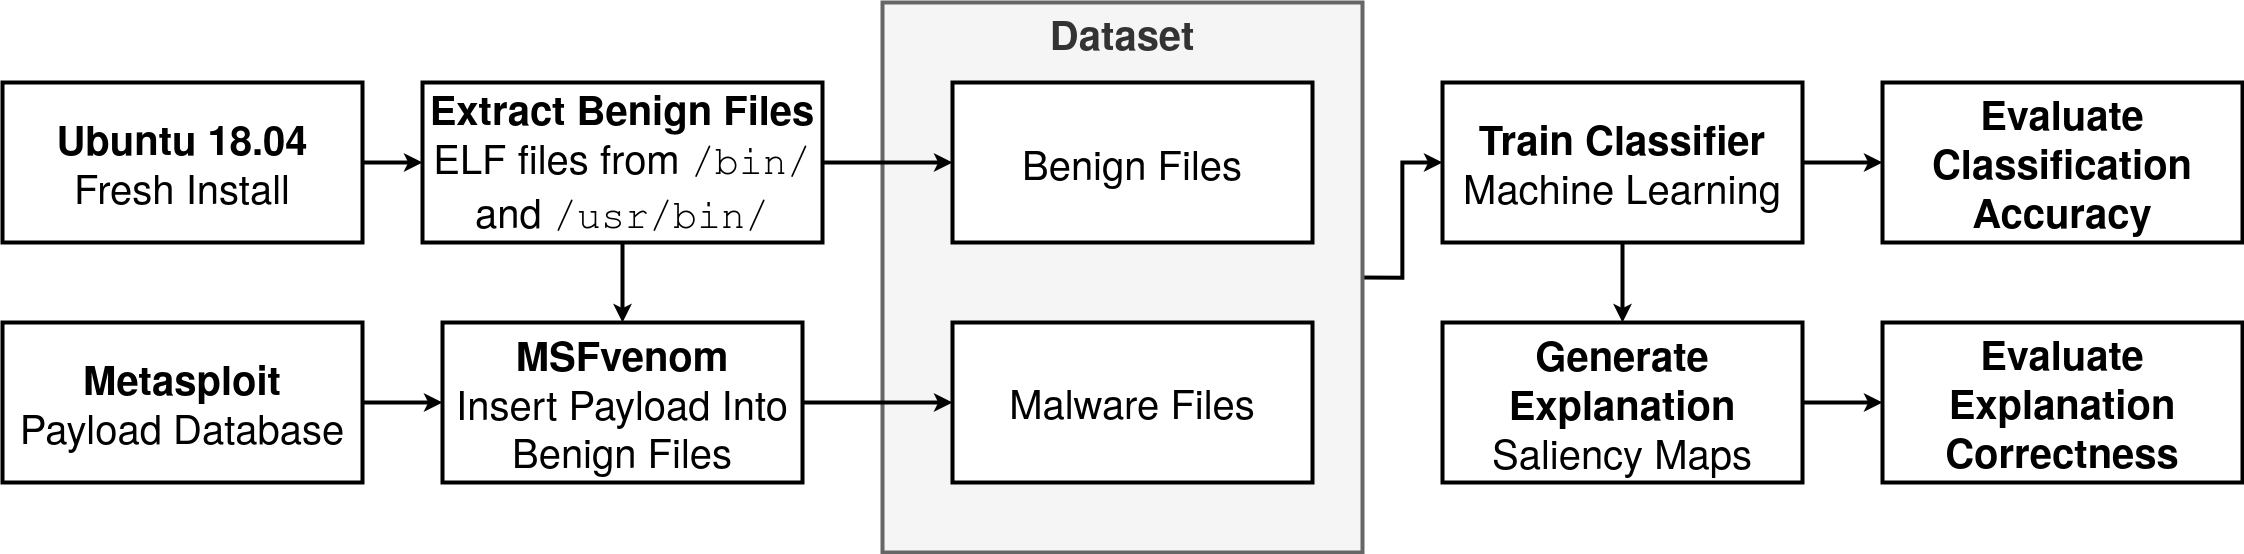
\includegraphics[width=\textwidth, keepaspectratio]{Images/Process_Overview_Diagram.png}
  \caption{Flow diagram showing methodology overview.}
  \label{fig:ProcessOverview}
\end{figure}

\subsection{Timeline}
The timeline for this project was shown in a Gantt chart.
The Fall schedule is found in \figRef{fig:GanttFall}, and the Spring schedule is found in \figRef{fig:GanttSpring}.

\begin{figure}[H]
  \centering
  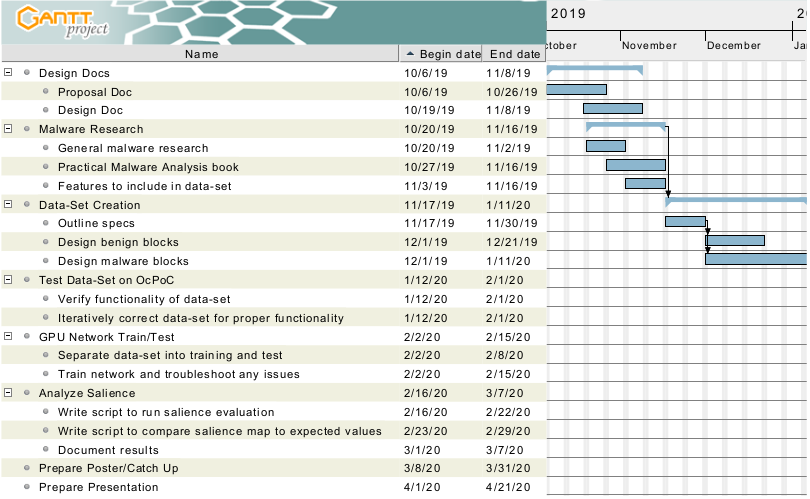
\includegraphics[width=\textwidth, keepaspectratio]{Images/Gantt_Chart_v2_Fall.png}
  \caption{Gantt chart showing Fall semester schedule.}
  \label{fig:GanttFall}
\end{figure}

\begin{figure}[H]
  \centering
  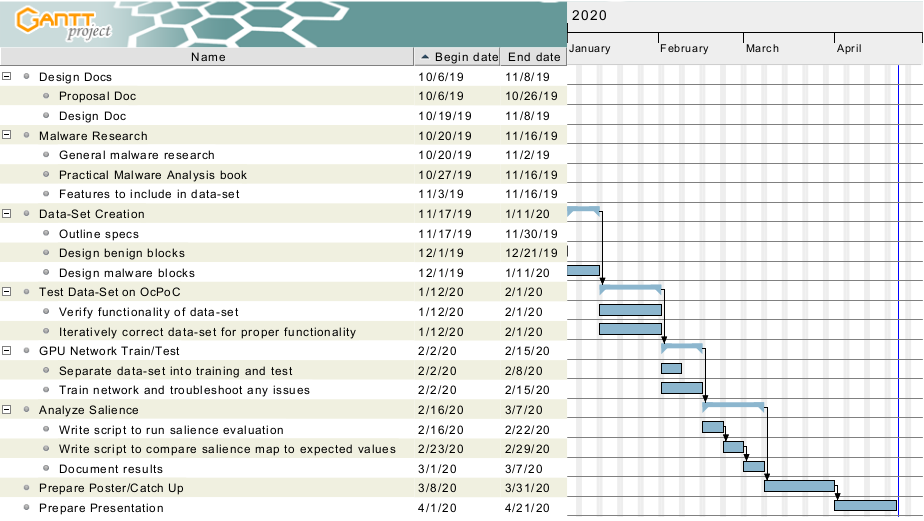
\includegraphics[width=\textwidth, keepaspectratio]{Images/Gantt_Chart_v2_Spring.png}
  \caption{Gantt chart showing Spring semester schedule.}
  \label{fig:GanttSpring}
\end{figure}

\pagebreak

\section{Methodology}
\subsection{Dataset Generation}
My method for dataset generation has two major goals.
The first goal is for the dataset to be easily interpretable for use in explainable machine learning.
In this case, interpretability means knowing which portion of the code is malicious and which is benign.
The second goal is for the method to be scalable to produce high volume datasets.

To meet these goals, I developed a dataset generation method consisting of two main stages.
The first stage involves gathering a pool of executable files, serving as the benign portion of the dataset.
In the second stage, a malicious Trojan is inserted into each benign file, forming the malware portion of the dataset.

\subsubsection{Gathering Benign Files}
I wanted my method of gathering benign files to be easily repeatable.
To achieve this goal, I gathered the benign files from a default installation of \ubu{} \ubuVer{}.
For convenience, the files were collected from an installation running on \vb{}, but the process can be replicated with a physical machine.
From this installation, I am interested in extracting executable binary files.
In the case of Linux, the most popular file format for executable files is the Executable and Linkable Format (ELF) \cite{ELF}.
In the Linux filesystem, many ELF files can be found in the \verb|/bin/| and \verb|/usr/bin/| directories.

\figRef{fig:ElfScraper} shows a bash script I wrote to scrape these directories for ELF files and copy them to the benign directories.
The script calls the \verb|find| command on both directories, which is a Unix program that searches through a given directory and outputs a list of files.
The \verb|file| command is called on each output, which displays information about the type of the file (i.e., "ASCII test" or "ELF 64-bit").
From this information, I filter out the ELF files with the \verb|grep| command, which is a command used to print out lines of a string or file matching a particular pattern.
In my case, I only want lines to display if the output of \verb|file| contains the string \verb|": ELF"|, designating it as an ELF file.
Each file from the filtered group is copied over to the directory designated by \verb|$BEN_DIR|, where they are stored for Trojan injection.
After gathering the benign pool, each file has the extension \verb|.benign| to distinguish from their infected counterparts.

\begin{figure}[H]
  \centering
  \lstinputlisting[language=bash, firstline=5]
  {"Code_Samples/elf_scraper.sh"}
  \caption{Bash script to scrape ELF files.}
  \label{fig:ElfScraper}
\end{figure}

\subsubsection{Trojan Insertion}
Once the benign files are collected, the malicious dataset is constructed by inserting a Trojan payload into each file.
To accomplish this task, I utilized the \metasploit{} \cite{Metasploit} framework.
\metasploit{} is a popular penetration testing framework containing payloads for various platforms, including Linux and Windows.
\msfv{}, a tool from the \metasploit{} framework, allows these payloads to be output in a variety of formats, but I am specifically interested in ELF format.
An extensive guide about the capabilities of \metasploit{} and \msfv{} can be found in \cite{MetasploitUnleashed}.

\figRef{fig:MsfCmd} shows an example command used to insert the payload into a sample file.
I specify the command to target the 64-bit Linux platform with a \payloadName{} payload.
This type of payload opens up a TCP port on the host machine and listens for an incoming connection from the attacker.
The template argument designates a file in which to insert the payload.
In this case, I insert the payload into the file \verb|ls.benign| and output the infected file to \verb|ls.infected|.

\begin{figure}[H]
  \centering
  \begin{lstlisting}[language=bash]
msfvenom --arch x64 --platform linux \
  --payload linux/x64/shell_bind_tcp LPORT=6666 \
  --format elf --out ls.infected \
  --template ls.benign
  \end{lstlisting}
\cprotect\caption{Example \msfv{} command call to insert a Trojan into \verb|ls.benign|.}
  \label{fig:MsfCmd}
\end{figure}

To automate the process of inserting the Trojan payload into every single benign file, I utilized the \verb|make| tool\cite{make}.
It is a versatile tool with the capability to automatically determine which components of a project require recompilation.
In typical usage, \verb|make| is used in conjunction with a build tool, such as \verb|gcc|.
A set of rules in a Makefile define parameters such as input files, output files, and specific commands needed to generate output files.
For my application, I treat \msfv{} as my build tool, files ending in \verb|.benign| as my source files, and files ending in \verb|.infected| as my output files.
The Makefile rules are configured so that if a \verb|.benign| file does not have a corresponding \verb|.infected| file, the \verb|.infected| file is generated by calling \msfv{} similarly to the command shown in \figRef{fig:MsfCmd}.

\subsection{Dataset Application}
In order to validate my dataset generation method, I used my dataset of \totalFiles{} files (\benignFiles{} of each class) in a malware classification task.
I chose to apply Malware as Image classification due to its ease of implementation.
I considered using Malware as Video due to Dr. Jha's lab's previous work exploring the technique \cite{SantacroceMaV, SantacroceSalience}.
However, due to the relative simplicity of implementing and analysing Malware as Image networks, I opted not to use Malware as Video for this example.
\figRef{fig:MaI} shows an overview of the Malware as Image method, including a visualization of the network architecture.
More specific network parameters will be discussed later.

\begin{figure}[H]
  \centering
  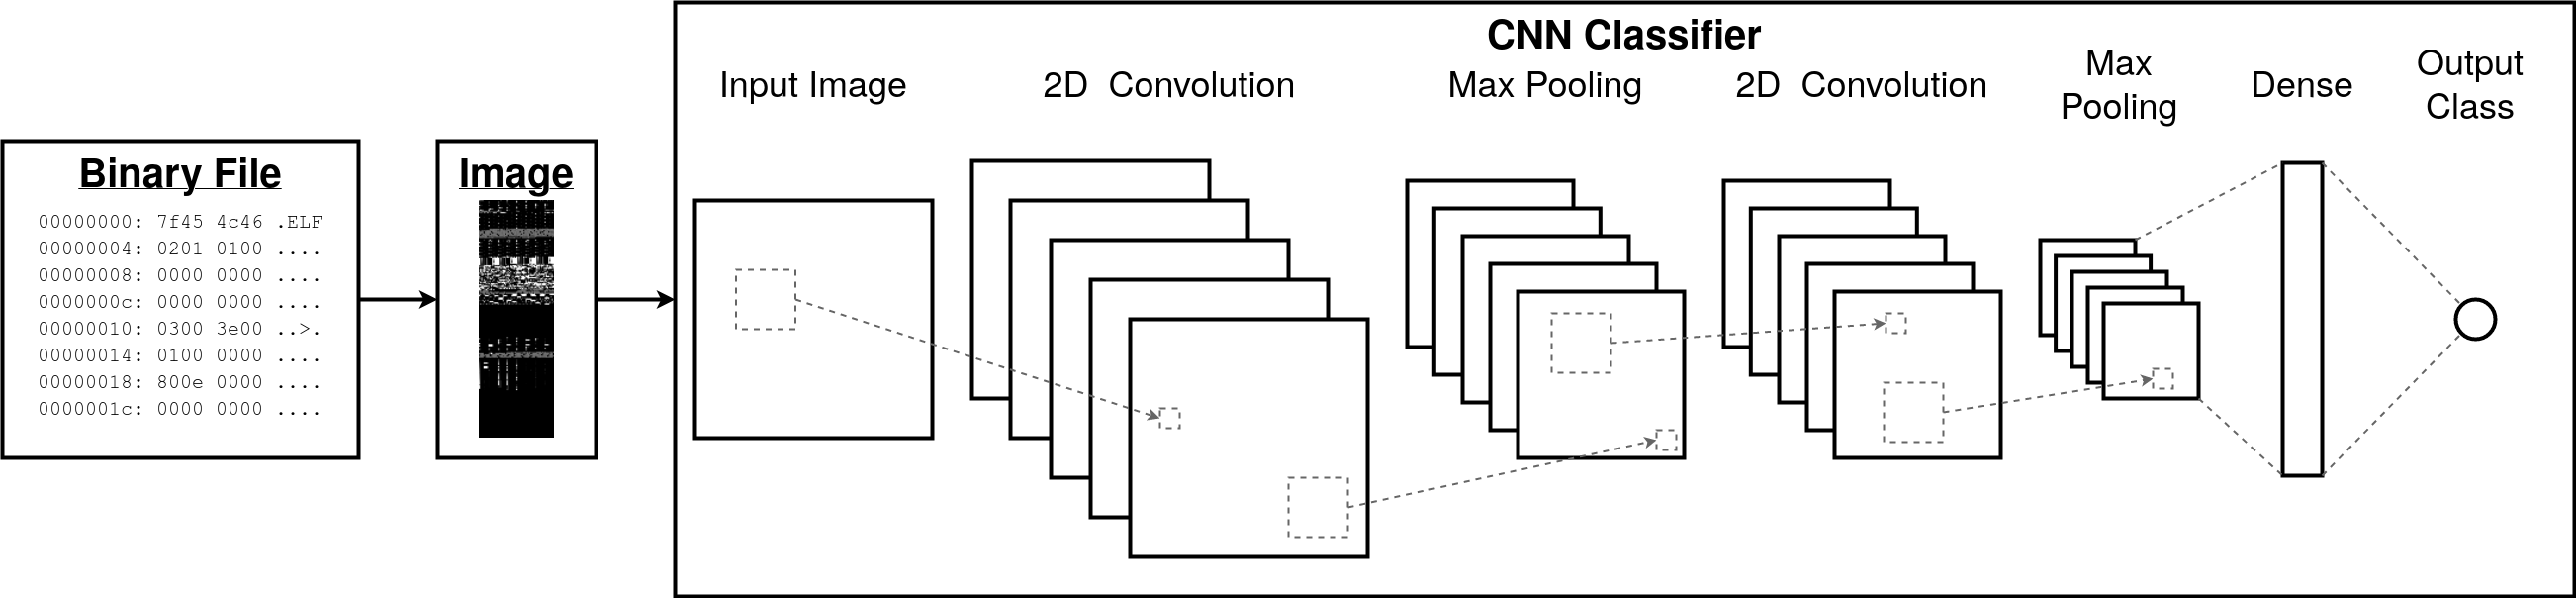
\includegraphics[width=\textwidth, keepaspectratio]{Images/Malware_as_Image.png}
  \caption{Overview of the Malware as Image classification model.}
  \label{fig:MaI}
\end{figure}

\subsubsection{Preprocessing}
To prepare the dataset for the network, the size of the image must be determined.
The network requires all inputs to have the same dimensions.
For simplicity, I simply pad the end of the files with zeros until they are all the same size.
To reduce the issue of having too much padding, I discard any files longer than \maxFileSize{}, leaving me with \usableFiles{} usable files.
\figRef{fig:FileSizeDist} shows the total amount of files at a given maximum file-size.
I then set the image width to \imageWidth{} pixels and the height to \imageHeight{} pixels.

\begin{figure}[H]
  \centering
  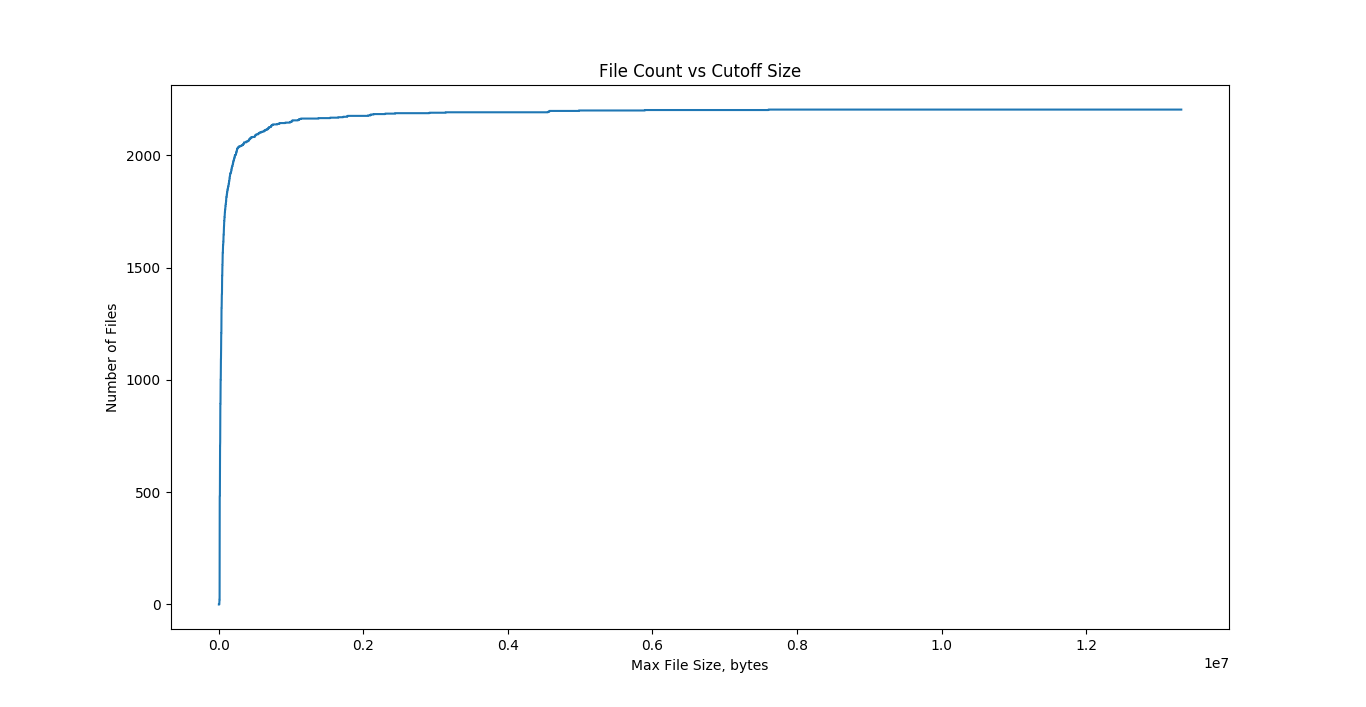
\includegraphics[width=\textwidth, keepaspectratio]{Images/file_size_vs_cutoff_size_all.png}
  \caption{Graph of File Count vs Maximum File-size.}
  \label{fig:FileSizeDist}
\end{figure}

Next, the binary file must be converted into an image file using methodology similar to \cite{Sgandurra}
I achieve this by first reading in the binary file as a byte array.
Each byte is then cast into an 8-bit unsigned integer, giving each element of the array an integer in the range [0, 255].
The array is then reshaped to have a width of \imageWidth{} and a height of \imageHeight{}, giving me a gray-scale image representation of the original binary file.
Note that during the reshaping process, the end of the file is padded with zeros to ensure it will fit the necessary dimensions.
\figRef{fig:FileImages} shows examples of image files generated from \verb|clear.benign| and \verb|clear.infected|.
Note that for space reasons, these images are 64 pixels wide and 200 pixels tall.

\begin{figure}[H]
  \centering
  \subfigure[]
  {
    
\includegraphics{Images/clear.benign.png}
  }
  \subfigure[]
  {
    
\includegraphics{Images/clear.infected.png}
  }
  \cprotect\caption{Example images: (a) \verb|clear.benign| (b) \verb|clear.infected|.}
  \label{fig:FileImages}
\end{figure}

\subsubsection{Classification}
To classify this dataset, I constructed a two-layer convolutional neural network similar to the one found in \cite{Sgandurra}.
\tabRef{tab:NetArch} shows the specific parameters for constructing my network.
The dataset was partitioned \trainPercent{} training data and \testPercent{} testing data.
I trained the network for \maxTrainingEpochs{} epochs with a batch size of \batchSize{}, a learning rate of \learningRate{}, and Binary Cross-entropy as the loss function.

\begin{table}[H]
  \caption{Malware Classification Network Architecture}
  \begin{center}
    \begin{tabular}{ccc}
      \hline
      \textbf{Layer Type} & \textbf{Activation} & \textbf{Notes}\\
      \hline
      2D Convolutional & tanh & Shape = 4x4\\
      \hline
      2D Max Pooling & N.A. & Shape = 3x3\\
      \hline
      Dropout & N.A. & Rate = 0.25\\
      \hline
      2D Convolutional & tanh & Shape = 3x3\\
      \hline
      2D Max Pooling & N.A. & Shape = 3x3\\
      \hline
      Dropout & N.A. & Rate = 0.25\\
      \hline
      Global Average Pooling & N.A. & N.A. \\
      \hline
      Dense & tanh & Size = 50\\
      \hline
      Dense & sigmoid & Size = 1\\
      \hline
    \end{tabular}
  \end{center}
  \label{tab:NetArch}
\end{table}

\pagebreak

\section{Results and Analysis}
\subsection{Dataset Generation}
My method is able to generate a dataset containing \benignFiles{} files of each benign and infected classes, totaling \totalFiles{} files.
Due to the nature of having both benign and infected versions of the same file, I am easily able to determine which features of the file are malicious and which are benign.
A simple diff of the infected file to the binary file will reveal this information, and it can be entirely automated.
The use of the \verb|make| command greatly helps to improve the scalability of the method.
Because the Makefile rules check which files need to be generated, it is possible to add a few files to the binary partition and have them quickly and automatically infected.

My dataset is greatly advantageous over the 2015 Microsoft Malware Classification Challenge dataset \cite{Ronen2018} in terms of intelligibility.
As previously discussed, I was unable to verify the benign and malicious components of the Microsoft dataset.
However, the malicious components of my dataset can easily be identified.
This level of intelligibility holds great promise to system verification of malware detection systems of any type.

An interesting behavior I observed from the infected files is that they do not actually run the Trojan payload.
This behavior is verified through the use of the \verb|netstat -atn| command.
The expected effect of running an infected file is for the port 6666 to open and listen for incoming connections.
However, running the infected file did not open any ports.
A "Trojan only" ELF file was generated by running the command from \figRef{fig:MsfCmd} without the template argument.
Running this file does cause the expected result of opening and listening on port 6666.
As seen in \figRef{fig:FileImages}, there is a section of code in \verb|clear.infected| that is not found in \verb|clear.benign| at the end of the file.
This code addition matches exactly with the "Trojan only" generated file, so I have confirmed that \msfv{} is inserting the actual Trojan into the template file.
I currently suspect that the lack of Trojan execution from the infected files is due to a glitch in the way \msfv{} modifies the entry-point of the code.
However, since the Trojan is actually inserted into the file, it can be found with static analysis.

\subsection{Malware Detection}
During the training process, I observed the training and validation accuracy over \maxTrainingEpochs{} epochs.
These observations are shown in \figRef{fig:AccVsEpochs}.
After training, the accuracy is \trainAccuracy{} on the training set and \testAccuracy{} on the validation set.
I observe that the training and validation accuracies flatten out after about 300-500 epochs.
While this result means that the network is likely overtrained, it does maintain a high validation accuracy throughout the entire duration of training.
Therefore, I have demonstrated the ability to use my new dataset for the purpose of training a malware detection machine learning algorithm.

\begin{figure}[H]
  \centering
  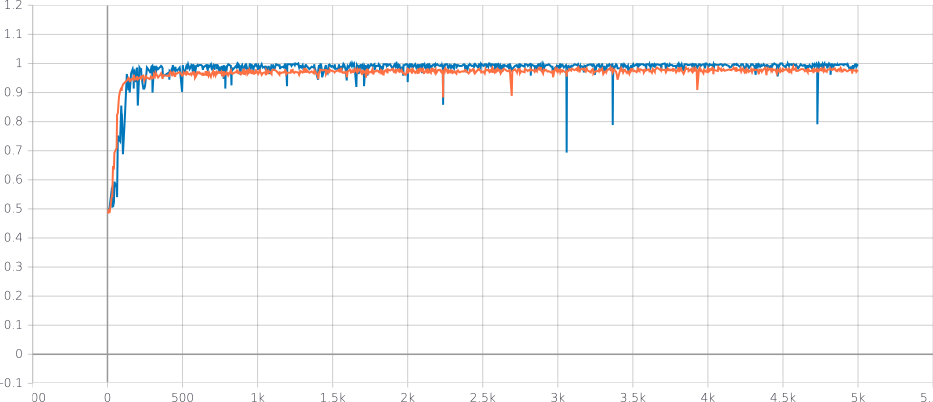
\includegraphics[width=\textwidth, keepaspectratio]{Images/epoch_accuracy_5k.png}
  \caption{Training (red) and validation (blue) accuracy over 5000 epochs.}
  \label{fig:AccVsEpochs}
\end{figure}

I used my network trained at \maxTrainingEpochs{} epochs and measured the performance.
These measurements are shown in \tabRef{tab:TestAcc}.
My network successfully classifies the entire training dataset correctly, and it only misses 1 file in the validation dataset.

\begin{table}[H]
  \caption{Malware Detection Results}
  \begin{center}
    \csvautotabular{Tables/acc_tab.csv}
  \end{center}
  \label{tab:TestAcc}
\end{table}

\pagebreak

\section{Conclusion}
My dataset generation method was able to successfully generate a dataset with features distinct enough to train a malware detection network to a testing accuracy of \testAccuracy{}.
My dataset is also intelligible as to specifically which features are malicious and which are benign.
Overall, my dataset generation method has shown promise to produce highly scalable datasets for machine learning.
In addition to malware detection, the explainable nature of the method allows the dataset to be used for tasks such as semantic segmentation of executable files.
The flexibility of the \metasploit{} framework allows this method to be extensible to virtually any target platform.

\subsection{Problems Encountered}
Throughout this project, I encountered many problems that I had to solve.
While some of these problems were able to be solved, I did not have time to resolve every issue.

One problem is that the training and validation processes were using a lot of memory.
The memory usage would scale linearly with the amount of files in the dataset.
The reason for this issue is that initially, I am transforming all of the files into images and storing them in memory before training began.
While the dataset generated for this work was a usable size, future considerations include the scalability of the dataset.
To resolve this problem, I can use the tensorflow.data.Dataset API.
This API allows custom mappings to be applied to datasets during training.
Using this technique, I can set the dataset to initially hold a list of file locations and provided a mapping function to transform the binary files into images, meaning only a single batch of data needs to fully load into memory at a time.
I have developed code to use this method in my digital image processing class, but I have not yet had time to port the solution to MiBeX.

The biggest ongoing issue is that the Trojans in the dataset do not activate.
I have done some troubleshooting on the matter, but have not been able to resolve it entirely.
First, I performed a binary file-diff on the benign and infected copies of the same file.
I verified that the Trojan was actually being inserted, and there is a small change at the beginning of the file.
I assume that the small change at the beginning is where \msfv{} changes the entry-point of the executable, but I have not verified this.
Next, I generated a stand-alone payload with \msfv{} and tested its functionality.
As expected with a \payloadName{} program, I used the \verb|netstat| command to observe that port 6666 was open and listening for incoming TCP packets while running the stand-alone payload.
Additionally, I verified that port 6666 does not open when running the infected file.
Further testing must be done to find the exact reason why the Trojan payload does not run in the infected files.

Another unresolved problem is getting TensorFlow 2.1 to generate image-specific class saliency maps.
I have found methods that other people have used to generate saliency maps with TensorFlow 2.1, but when I attempt to implement them I receive error messages about the input dimensionality.
Unfortunately, I have not had time to resolve these errors.

\subsection{Future Recommendations}
The first future recommendation is to fix the issue with TensorFlow and calculating the saliency maps.
Completing this task will help to round out the story presented by this project and fully realize the proof of concept malware detection application.

The most obvious limitation with this dataset generation method is that the Trojan does not actually run.
While this limit still allows the dataset to be used for static analysis, it is completely unusable for dynamic analysis.
Fixing this issue is the largest area of improvement for this method.
Another interesting area of improvement is adjusting where the Trojan payload is inserted into the file.
With \msfv{}, the Trojan is always inserted at the end of the file.
However, investigating different padding methods might make the Trojan appear to be in the middle of the file instead of the end.

This method can be expanded upon in several ways.
While this work only demonstrates the creation of a two-class dataset, \msfv{} can be configured to insert many different types of Trojan payloads.
In fact, \msfv{} has the capability to use custom payloads, as well as payload obfuscation techniques.
\msfv{} has the tools available to produce an extremely diverse dataset.
The only limiting factor is the amount of payloads that can be found.
Increasing the diversity of the types of Trojan payloads will prove beneficial to further testing the performance of various classification techniques.
I can also expand upon the size of the dataset by adding more benign files.
\ubu{} has a vast collection of files in its software repositories which can be freely downloaded and added to the benign set.

\pagebreak

% Bibliography
\bibliographystyle{ieeetr}
\bibliography{references}

\pagebreak

\appendix
\section{Code}
All of the code for this project can be found at https://github.com/stegnerw/MiBeX.

\subsection{Dataset Generation}

\cprotect\subsubsection{\verb|elf_scraper.sh|}

\lstinputlisting[language=bash]
{"Code_Samples/elf_scraper.sh"}

\cprotect\subsubsection{\verb|Makefile|}

\lstinputlisting[language=make]
{"Code_Samples/Makefile"}

\subsection{Malware as Image Classifier}

\cprotect\subsubsection{\verb|file_size_analysis.py|}

\lstinputlisting[language=Python]
{"Code_Samples/file_size_analysis.py"}
\cprotect\subsubsection{\verb|FileImage.py|}

\lstinputlisting[language=Python]
{"Code_Samples/FileImage.py"}

\cprotect\subsubsection{\verb|partition_dataset.py|}

\lstinputlisting[language=Python]
{"Code_Samples/partition_dataset.py"}

\cprotect\subsubsection{\verb|pickle_dataset.py|}

\lstinputlisting[language=Python]
{"Code_Samples/pickle_dataset.py"}

\cprotect\subsubsection{\verb|train_cnn_v1.py|}

\lstinputlisting[language=Python]
{"Code_Samples/train_cnn_v1.py"}

\end{document}

